\documentclass[a4paper,11pt]{article}
\usepackage[utf8]{inputenc}
\usepackage[T1]{fontenc}
\usepackage[a4paper,top=2.2cm,bottom=2.2cm,left=2.1cm,right=2.1cm]{geometry}
\usepackage{lmodern,microtype}
\usepackage{amsmath,amssymb,graphicx,booktabs,tabularx,longtable,array}
\usepackage{enumitem,xcolor,tikz,caption,fancyhdr}
\usepackage{hyperref}
\usetikzlibrary{positioning,arrows.meta,fit}
\definecolor{navy}{RGB}{28,55,86}
\definecolor{softblue}{RGB}{241,246,251}
\hypersetup{colorlinks=true,linkcolor=navy,urlcolor=navy,citecolor=navy,
  pdftitle={Acoustic Mosquito Species Classification on ESP32-S3},pdfauthor={Minh Luan Vo}}
\setlist{itemsep=2pt,topsep=4pt,leftmargin=1.5em}
\newcolumntype{Y}{>{\raggedright\arraybackslash}X}
\newcolumntype{P}[1]{>{\raggedright\arraybackslash}p{#1}}
\renewcommand{\arraystretch}{1.17}
\captionsetup{font=small,labelfont=bf,skip=7pt}
\setlength{\parskip}{4pt}
\setlength{\parindent}{0pt}
\setlength{\headheight}{15pt}
\setlength{\emergencystretch}{1.5em}
\setcounter{tocdepth}{1}
\pagestyle{fancy}
\fancyhf{}
\fancyhead[L]{\small Acoustic Mosquito Edge AI\enspace|\enspace Research Proposal}
\fancyhead[R]{\small Minh Luan Vo}
\fancyfoot[C]{\thepage}
\newcommand{\core}{\textbf{Core}}
\newcommand{\advanced}{\textbf{Optional extension}}

\begin{document}
\begin{titlepage}
\centering
\vspace*{0.9cm}
{\Large\bfseries VIETNAMESE-GERMAN UNIVERSITY}\\[0.3cm]
{\large Computer Science and Engineering}\\[1.6cm]
{\Large\textsc{Research Proposal}}\\[0.7cm]
{\color{navy}\rule{\linewidth}{0.7mm}}\\[0.55cm]
{\LARGE\bfseries Acoustic Mosquito Species Classification\\[0.2cm]
on ESP32-S3}\\[0.5cm]
{\large A Real-Time TinyML Core with an Optional\\[0.12cm]
Synthetic-Overlap Research Extension}\\[0.55cm]
{\color{navy}\rule{\linewidth}{0.7mm}}\\[1.15cm]
\begin{minipage}[t]{0.46\textwidth}\raggedright\large
\textbf{Prepared by}\\[0.15cm]Minh Luan Vo\\[0.55cm]
\textbf{Program}\\[0.15cm]Computer Science and Engineering
\end{minipage}\hfill
\begin{minipage}[t]{0.46\textwidth}\raggedright\large
\textbf{Supervisor}\\[0.15cm]Dr. Vo Bich Hien\\[0.55cm]
\textbf{Proposed duration}\\[0.15cm]12 weeks
\end{minipage}
\vfill
\begin{minipage}{0.9\textwidth}\centering
\textbf{Completion principle:} the deployed single-mosquito classifier and its evaluation constitute the complete core project. Synthetic-swarm experiments are conditional on core completion.
\end{minipage}\\[0.8cm]
{\large September 2026}
\end{titlepage}

\pagenumbering{roman}
\begin{abstract}
This project investigates whether a mosquito acoustic species classifier can be compressed and deployed for real-time local species inference from mosquito-active audio on an ESP32-S3 while retaining useful classification performance. The mandatory core uses real recordings of individually recorded mosquitoes, a compact audio representation, and a lightweight classifier trained off-device. The ESP32-S3 will acquire microphone audio, compute matching features, execute the exported model, and produce predictions. Evaluation will measure species classification, changes after INT8 quantization, model and firmware size, runtime memory, processing time, and continuity of acquisition. The contribution is a reproducible engineering study of classification--resource trade-offs, rather than a claim of a new mosquito recognition algorithm.

The core is a closed-set species-classification task on mosquito-active audio from a small, fixed species set. It does not establish general mosquito/background detection, species identification outside that set, or mosquito abundance. Dataset selection and source grouping will be audited before windowing, and all model selection and calibration will remain separate from final testing. Continuous audio acquisition with periodic closed-set species inference will be demonstrated using controlled playback of held-out real single-mosquito recordings; this tests the physical acquisition chain without being represented as live-insect field validation or general mosquito/background detection.

Only after the core is complete will an optional study compare a reconstruction of the author's previous synthetic-overlap strategy with a revised generator. The revised generator will emphasize active source segments, controlled overlap and relative levels, environmental noise, and source-disjoint evaluation. Both conditions will use the same compact multi-label model and preprocessing. Improvements on synthetic tests will be distinguished from improvements through a physical playback channel, and neither will establish transfer to natural swarms.

The three available real swarm recordings, each approximately 12 seconds long, will remain excluded from training and tuning. They can support only a final qualitative case study: their number is very small, acquisition was uncontrolled, and biological presence does not establish acoustic activity in every analysis window. The twelve-week plan prioritizes early hardware checks and core evaluation, protects time for reporting, and allows the extension to be omitted or reported as a negative result.
\end{abstract}
\vspace{0.3cm}
\tableofcontents
\clearpage
\pagenumbering{arabic}

\section{Research Problem, Questions, and Scope}
\subsection{Motivation and contribution}
Mosquito flight recordings contain information useful for distinguishing some species, but acoustic signatures also vary with sex, individual, and recording conditions. The Abuzz study established smartphone-based acoustic collection and classification; it did not establish universally separable species signatures \cite{abuzz}. MosquitoSong+ studied classification with environmental-noise and signal-level augmentation \cite{mosquitosong}. These results motivate a limited acoustic classifier, not a replacement for taxonomic identification or a validated surveillance instrument.

Altayeb et al. demonstrated mosquito wingbeat classification with TinyML on embedded hardware \cite{tinyml}. The remaining student-scale task is to connect a defensible evaluation protocol to the entire ESP32-S3 acquisition, preprocessing, and inference chain. Training will occur on a computer; deployment will require no remote inference. The engineering contribution is the measured trade-off among classification quality, memory, storage, and sustained processing speed on this particular platform.

The optional research hypothesis is that better-controlled synthetic overlap may improve multi-label detection under held-out overlap and acquisition conditions. This extends the author's \textit{Synthetic Swarm Mosquito Dataset for Acoustic Classification: A Proof of Concept} \cite{previous}. Linear mixing, compact CNNs, and quantization are established methods. Whether the proposed changes improve transfer is an experimental question, not an expected finding.

\subsection{Questions and evidence}
\begin{table}[htbp]
\centering\small
\caption{Research questions and the experiments that can answer them.}
\label{tab:rq}
\begin{tabularx}{\linewidth}{P{1.3cm}Y Y}
\toprule
 & \textbf{Question} & \textbf{Required evidence}\\\midrule
RQ1\newline Core & Can a compact closed-set species classifier perform real-time inference on mosquito-active audio on ESP32-S3 with acceptable loss of classification performance? & Group-disjoint offline evaluation; paired FP32/INT8 comparison; on-device numerical checks and sustained microphone inference.\\
RQ2\newline Core & What classification--resource trade-offs and sensitivity to added noise arise in the selected pipeline? & One reference and one compact configuration; model/firmware size, RAM and pipeline timing; fixed held-out environmental-noise test.\\
RQ3\newline Optional & Does revised synthetic overlap improve multi-label species detection beyond the training generator, and can the model fit the same edge platform? & Matched generator comparison on unseen-source mixtures and a fixed stress test; playback if time permits; INT8 and device profiling if attempted.\\
\bottomrule
\end{tabularx}
\end{table}

\subsection{Task boundaries and completion}
\core{} comprises a documented baseline replication, leakage-safe data partitions, a compact classifier, quantization, ESP32-S3 deployment, continuous audio acquisition with periodic species inference, and classification and hardware measurements. Its target is a \emph{known species given suitable mosquito-active audio}. The output is a species score vector, with an ``insufficient signal'' status for silence, clipping, or acquisition faults. That status is a signal-quality check, not a trained mosquito detector. A confident species output on background or an unknown species can still be wrong.

\advanced{} comprises a bounded comparison of two synthetic generators and a sigmoid multi-label classifier. Embedded swarm inference, playback, and the final three-recording case study are further conditional stages. None is necessary for core completion. The study excludes source separation, mosquito counting, clinical/public-health effectiveness, and a claim of field-ready surveillance. A laptop-only model or stored-input MCU demonstration is an intermediate result; full core completion requires continuous inference from the microphone.

All numerical settings below are \emph{proposed experimental settings or engineering targets}, not measured results or literature-derived performance guarantees. Feasibility depends on access to usable recordings and working hardware; those dependencies are checked in the first two weeks.

\section{Evidence Base and Dataset Protocol}
\subsection{Dataset selection and label suitability}
The preferred primary resource is the \textbf{Tiny MosquitoSong dataset released with MosquitoSong+}. Its authors describe individual mosquitoes placed in small net cages and recordings of \textit{Aedes aegypti}, \textit{Aedes albopictus}, \textit{Anopheles dirus}, and \textit{Culex quinquefasciatus}, with sex labels and environmental-noise files \cite{mosquitosongdata}. This directly matches the intended single-mosquito core more closely than an unspecified mixture of public corpora.

Before adopting it, the project will verify access, clip duration, original-recording relationships, and whether multiple files or channels come from the same individual/session. Its documented individual collection procedure does \emph{not} establish that usable individual IDs are present in the released files. Pre-segmented overlapping epochs must be traced to their original source. If those relationships cannot be recovered, those epochs will not be randomly split and presented as independent test examples.

\begin{table}[htbp]
\centering\small
\caption{Roles of other public resources; inclusion is conditional on provenance and label compatibility.}
\label{tab:data}
\begin{tabularx}{\linewidth}{P{2.6cm}Y Y}
\toprule
\textbf{Resource} & \textbf{Appropriate use} & \textbf{Restriction}\\\midrule
HumBugDB \cite{humbug} & Fallback primary subset, especially documented individually recorded cup data; annotated mosquito events can help source selection. & Use species-labelled, provenance-traceable subsets only. Detection annotations, species labels, and individual identity are different metadata.\\
Abuzz \cite{abuzz,abuzzdata} & Historical source of the previous paper; possible secondary single-species transfer check. & Cage recordings following a flying mosquito do not certify every recording as isolated single-individual audio. Do not infer individual identity from a file alone.\\
BioDCASE 2026 Task 5 \cite{biodcase} & Context for domain shift; optional compatible external evaluation. & Cross-domain species classification is not a mixed-species swarm benchmark. Check species intersections, provenance overlap, and test-label availability first.\\
\bottomrule
\end{tabularx}
\end{table}

The week-two data gate will retain two to four species with sufficient independent source groups in each partition. The preferred four-species set is named above; any reduction will follow group availability and training/validation evidence before final testing. The report will retain exact species names rather than replace them with genus labels. Sex, device, and session distributions will be recorded when available; a class confounded with one device or one sex will be restricted or explicitly acknowledged. Corpora will not be pooled merely to increase sample count.

If the preferred release lacks recoverable source groups or suitable durations, the fallback is a documented single-individual HumBugDB subset, with a smaller species set if necessary. If neither provides independent labelled data, supervisor review is required at week two; creating many windows cannot repair a lack of independent recordings. Dataset versions, provenance, permitted use, exclusions, and group counts will be recorded. No new large live-mosquito collection is a core dependency.

\subsection{Partition before windowing or augmentation}
Use one reproducible, approximately 60/20/20 training/validation/test split \emph{by independent groups}, balancing species as far as the group structure permits. Group all recordings linked to the same known individual or session; where these IDs are absent, use the original recording and known acquisition batches. Duplicate audio, re-exports, overlapping snippets, and paired microphone channels must remain together. Never invent individual or session IDs. Recording-disjoint testing with unknown individual identity will be described as such, with residual dependence acknowledged.

The split manifest will be fixed before extracting windows. It will show species, available metadata, group assignments, durations, and exclusion reasons. Exact hashes and near-duplicate/source-overlap checks will reduce accidental duplication. Window count will not be substituted for the number of independent test groups. All crops, augmented versions, and synthetic mixtures inherit their source partition. Noise recordings are partitioned by original file/session as well, including when shared by more than one dataset.

Feature statistics, class weights, activity-rule parameters, and INT8 calibration examples come from training data only. Architecture selection, early stopping, and decision thresholds use validation data. The final test set, external test recordings, and three real swarm recordings never participate in these choices. If independent groups are sparse, report that limitation and group-wise validation variation instead of creating a misleadingly large window-level benchmark.

\subsection{Activity, background, and evaluation units}
Prefer annotated wingbeat intervals. Otherwise, inspect training audio and spectrograms to define a simple fixed activity/quality rule, then apply it unchanged to each partition. Report accepted duration and rejection rates per species, and audit a sample without changing the frozen rule after seeing test performance. Silence or unrelated noise must not acquire a species label simply because it occurs in a species-labelled file. Short clips will not be looped or concatenated across sources to manufacture independent examples.

A separate background collection supports noise tests and an exploratory description of erroneous species outputs. It does not automatically provide comprehensive negative examples for a mosquito detector. Adding a supervised background detector would require independently labelled negatives, separate validation, and its own performance claims; it is outside the mandatory scope.

\section{Core Methodology and Evaluation}
\subsection{System design and early hardware verification}
\begin{figure}[htbp]
\centering
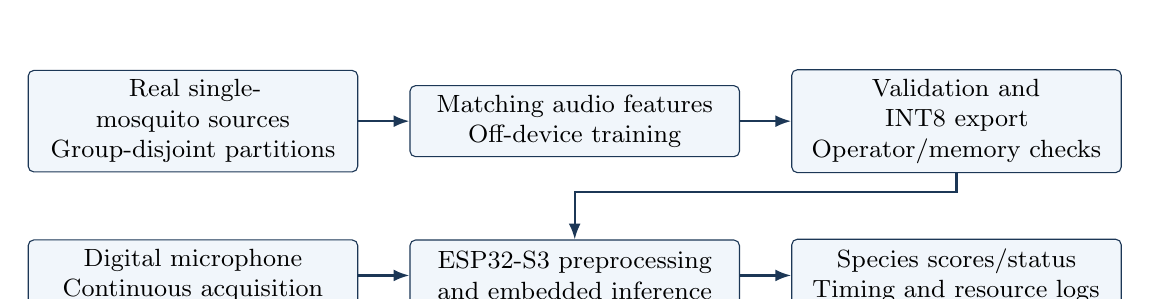
\begin{tikzpicture}[
  box/.style={draw=navy,fill=softblue,rounded corners=2pt,align=center,text width=3.95cm,minimum height=0.9cm,font=\small},
  arr/.style={-{Latex[length=2mm]},thick,draw=navy},node distance=0.6cm and 0.65cm]
\node[box] (data) {Real single-mosquito sources\\Group-disjoint partitions};
\node[box,right=of data] (train) {Matching audio features\\Off-device training};
\node[box,right=of train] (export) {Validation and INT8 export\\Operator/memory checks};
\node[box,below=0.85cm of data] (mic) {Digital microphone\\Continuous acquisition};
\node[box,right=of mic] (dsp) {ESP32-S3 preprocessing\\and embedded inference};
\node[box,right=of dsp] (out) {Species scores/status\\Timing and resource logs};
\draw[arr] (data)--(train);\draw[arr] (train)--(export);
\draw[arr] (mic)--(dsp);\draw[arr] (dsp)--(out);
\draw[arr] (export.south) -- ++(0,-0.24) -| (dsp.north);
\end{tikzpicture}
\caption{Mandatory pipeline. Training is off-device; the complete microphone-to-prediction path runs on ESP32-S3. Synthetic overlap is a later experiment.}
\label{fig:pipeline}
\end{figure}

The ESP32-S3 provides dual-core processing up to 240~MHz, 512~KB on-chip SRAM, and I2S support \cite{espdatasheet}. These chip specifications do not describe free application RAM or the flash/PSRAM fitted to a particular board. Week one will record the actual board variant, microphone, clock, usable memory, and software versions. A minimal acquisition and small-model inference test will verify audio format, buffer continuity, supported operators, and tensor allocation before extensive training. External PSRAM, if used, will be reported separately rather than treated as on-chip SRAM.

The intended runtime is Espressif's TensorFlow Lite Micro integration with supported ESP-NN kernels \cite{esptflm}. Accelerated kernels can help, but the latency of an unrelated demonstration is not a forecast for this model. The project will use existing inference and DSP libraries and avoid developing a new runtime, custom neural-network operators, or a user interface beyond local/serial prediction output.

\subsection{A fixed, compact audio front end}
Table~\ref{tab:dsp} specifies an initial design to make the experiments concrete. It is an engineering starting point, not a claim that Mel features or these parameters are optimal for mosquitoes. Training-only spectral inspection and an initial MCU profile will confirm or revise it before the core comparison is frozen.

\begin{table}[htbp]
\centering\small
\caption{Proposed baseline preprocessing contract, shared by training and deployment.}
\label{tab:dsp}
\begin{tabularx}{\linewidth}{P{3.2cm}Y}
\toprule\textbf{Item} & \textbf{Initial setting and rationale}\\\midrule
Audio input & Mono, 16~kHz; fixed PCM scaling. Offline resampling uses anti-alias filtering. The microphone path must supply the same effective rate and scaling.\\
Context and update & 1.0~s rolling context; one prediction every 0.5~s. The duration audit may reduce context to 0.5~s before model selection if real active clips are too short. No cross-source concatenation.\\
STFT & 512-sample Hann analysis window, 512-point FFT, 256-sample hop, no centred padding. At 16~kHz: 32~ms windows, 16~ms hops, 31.25~Hz bin spacing.\\
Features & Power spectrum, 40 Mel-spaced filter-bank energies over 100--4000~Hz, then a fixed-floor logarithm. This band is provisional; inspect training spectra for excluded useful harmonics.\\
Tensor and scaling & A 1~s context gives $1+\lfloor(16000-512)/256\rfloor=61$ frames: $40\times61\times1$. Training-fitted feature normalization is frozen. A 0.5~s context gives 30 frames.\\
Parity details & Fix Hann convention, FFT/power normalization, Mel formula and filter normalization, log floor/base, feature scaling, frame alignment, input quantization, and treatment of startup/incomplete frames.\\
\bottomrule
\end{tabularx}
\end{table}

Here, Mel-filter-bank energies (MFE) and their logarithms are stages of one feature pipeline, not automatically different experiments. MFCCs apply a cepstral transform to log filter-bank energies and may discard detail if only a few coefficients are retained. A log-STFT preserves linear-frequency bins but may require a larger tensor. No general ranking among these representations is assumed.

If resources and time allow \emph{one} comparison, evaluate log-power STFT bins over the same band against log-Mel, retaining the same context, split, training budget, and CNN family. Report changes in input dimensions, parameters, operations, and RAM so unequal computational cost is visible. A larger FFT or MFCC study is a fallback investigation only if evidence identifies a specific resolution or memory problem. Frequency-bin spacing is not equivalent to the ability to resolve two tones; window duration and leakage also matter. A $224\times224$ RGB rendering, colour map, or image resize adds no independent acoustic channels and is unnecessary for the mandatory embedded tensor.

Remove DC consistently and check clipping and input quality, but avoid adaptive denoising, pitch changes, or unvalidated harmonic enhancement. Do not normalize every window to its own peak or RMS when testing level sensitivity: this can erase the variable under test. Fixed PCM scaling and frozen feature normalization preserve a defined amplitude reference; any automatic microphone gain must be disabled or documented.

\subsection{Baseline, compact classifier, and quantization}
First reproduce the \emph{method} of a published TinyML mosquito baseline using the reported feature/model configuration and available implementation \cite{tinyml}. Document departures required by the selected data and group-safe split. Scores obtained under a different partition or species set are not an exact reproduction of the published score. If the full historical configuration cannot be recovered, identify the result as a documented reimplementation, not an exact replication.

The edge candidate will be a small convolutional network with at most three convolution/pooling stages, global average pooling, and a $K$-way softmax head. Start with narrow channels and supported operators; reduce width or input size if profiling demands it. One reference and one compact configuration are sufficient. Do not conduct a broad architecture search or inherit ResNet-18/LSTM backbones simply because the previous study used them. The model is trained off-device with categorical cross-entropy:
\begin{equation}
 p_k=\frac{\exp(z_k)}{\sum_{j=1}^{K}\exp(z_j)},\qquad
 \mathcal{L}_{\mathrm{single}}=-\sum_{k=1}^{K}y_k\log p_k .
\end{equation}
Here $\mathbf{y}$ is one-hot and $K$ is the fixed number of selected species. Class balancing is computed from training data, and early stopping uses validation macro-F1 or loss under one stated rule. Repeat the selected compact configuration with three training seeds; choose the deployable checkpoint by validation performance subject to resource limits, not by its test score.

Export the selected model and attempt full INT8 post-training quantization with representative training features, including training-only level/noise variation \cite{quantization}. Verify operator coverage and integer tensors rather than equating a small file with full integer inference. DSP may remain floating point if its measured cost fits; ``INT8 model'' does not imply an all-integer acquisition/front end. Quantization-aware training is a bounded fallback if the validation loss of performance remains unacceptable after calibration and simplification.

The comparison chain is FP32 training model, exported FP32 model, host INT8 model, and MCU INT8 model. Feed identical known PCM through both front ends, then compare features, quantized tensors, scores, and decisions. Use development fixtures to establish expected numerical tolerances before testing. Report maximum feature/score deviations and decision disagreements, investigating systematic differences rather than assuming bit-identical floating-point DSP. Physical playback is a separate channel experiment, not a numerical parity test.

\subsection{Classification and robustness evaluation}
The primary species metric is macro-F1; also report balanced accuracy, per-species precision/recall/F1, the confusion matrix, and the number of independent groups. Use the same held-out windows for paired FP32/INT8 comparisons and express score loss in percentage points. Report both window-level results and group-aggregated results, so long recordings do not dominate. A class-prior baseline provides context. Resample original groups, not windows, for approximate confidence intervals when group counts support them; with few groups, emphasize counts and descriptive variability rather than strong significance claims.

The core robustness test adds held-out environmental noise at nominal recording-to-added-noise ratios of 20, 10, and 0~dB, alongside unmodified audio. These are controlled stress levels, not measurements of natural mosquito SNR. With source recording $s$ and noise $n$, choose $\alpha$ for a target ratio $R$ using
\begin{equation}
 R=10\log_{10}\frac{P_s}{\alpha^2 P_n},\qquad x=s+\alpha n.
 \label{eq:ratio}
\end{equation}
Powers use the documented active interval. Since $s$ already contains acquisition noise, $P_s$ is not clean wingbeat power. Use common attenuation of the completed mixture where necessary to avoid clipping, record it, and do not independently normalize its components afterwards. Test conditions and seeds are fixed before final evaluation. If amplitude sensitivity is also measured, use separate fixed input attenuations and hold added noise constant; this is not a physical distance experiment.

\subsection{Embedded measurements and completion gate}
The device processes rolling audio while acquisition continues. Let $H=0.5$~s be the update interval and $T_{\mathrm{step}}$ the elapsed time for preprocessing, inference, and decision/output work for one update. Define
\begin{equation}
 \mathrm{RTF}_{\mathrm{update}}=\frac{T_{\mathrm{step}}}{H}.
\end{equation}
Sustained real time requires keeping up with the \emph{update interval}, not merely finishing within the 1~s context. Report DSP time, inference time, total step time, median, 95th percentile, observed maximum, deadline misses, and dropped samples/buffer overruns. The first output also requires filling the context; processing latency must be distinguished from observation delay.

\begin{table}[htbp]
\centering\small
\caption{Core evidence and engineering targets. Targets are proposed, not promised outcomes.}
\label{tab:gate}
\begin{tabularx}{\linewidth}{P{3.0cm}Y}
\toprule\textbf{Dimension} & \textbf{Evidence / gate}\\\midrule
Classification & Aim for compact INT8 macro-F1 within 5 percentage points of the reproduced FP32 reference and within 3 points of its own FP32 version. Report absolute and per-class scores even if these relative targets are met.\\
Resource fit & Model allocation and firmware fit the measured board budget. Report serialized model bytes, complete firmware/partition usage, tensor arena, DSP/audio buffers, stack/heap high-water estimates, and internal/external RAM separately. Target at least 20\% headroom against measured usable application budgets.\\
Continuous operation & A 30-minute microphone run with no observed lost audio, overruns, crashes, or missed 0.5~s update deadlines. Report the full run length and counts; this is a prototype stability check, not long-term reliability evidence.\\
Physical input & Re-record held-out single-mosquito audio through a loudspeaker and the actual microphone at documented fixed geometry and levels. Include quiet/background periods and disclose the channel-induced classification change.\\
Measurement limits & Power is optional only with a suitable current measurement setup; state supply, clock, radio state, and measurement scope. Do not infer battery lifetime from model size.\\
\bottomrule
\end{tabularx}
\end{table}

The relative F1 targets do not make a weak reference scientifically useful. By week three, the supervisor and student will record a minimum validation macro-F1 and per-class recall requirement informed by the reproduced baseline and class support, before final-test access. If meaningful discrimination is absent, revise labels/features or narrow scope while preserving an untouched test set. The stated 5/3-point targets are engineering tolerances, not universal biological requirements; failing a target is reported honestly.

Microphone playback demonstrates the full local sensing-to-inference chain and acoustic channel sensitivity. The played species is known, but audibility is checked rather than assumed. The loudspeaker response and gain can alter flight tones; digital predictions and re-recorded predictions are compared on paired source clips. This is not a genuine live-insect test and does not establish field accuracy. A supervised live single-mosquito demonstration may supplement it if practical, without becoming a data-collection dependency.

\section{Optional Synthetic-Overlap Research Extension}
\subsection{Entry condition and multi-label task}
Begin only after the core pipeline, measurements, and core report draft are complete. The first extension is deliberately small: two generators, one fixed lightweight model, and a held-out-source test plus one fixed stress condition. If it cannot be completed within the reserved time, retain the core as the final project and document any partial extension separately.

For each analysis window, $y_k=1$ means that an eligible active source of species $k$ contributes within that window under the declared synthesis rule. Multiple species may be positive. Use independent logits and a numerically stable binary cross-entropy loss:
\begin{equation}
 p_k=\sigma(z_k),\quad
 \mathcal{L}_{\mathrm{multi}}=-\frac{1}{K}\sum_{k=1}^{K}
 \left[y_k\log p_k+(1-y_k)\log(1-p_k)\right].
\end{equation}
An implementation using a logits-based loss consumes $z_k$ directly; sigmoid is not applied twice. Source multiplicity is retained as synthesis metadata only. This is species-presence classification, not source separation or a count estimator.

Choose one global decision threshold on validation macro-F1 using a fixed grid from 0.1 to 0.9 in steps of 0.05; break ties in favour of the higher threshold. Freeze it before the final tests. Per-species thresholds are optional only if validation support is adequate. Report macro-/micro-F1, per-species precision/recall, average precision, label prevalence, and background-only false-positive behaviour. Show threshold sensitivity on validation data; never choose a better threshold from final synthetic, playback, or real-swarm results. A post hoc threshold changes decisions, not the loss of an unchanged trained model.

\subsection{Two controlled generators}
The mixture model is a first-order superposition of recorded signals:
\begin{equation}
 x[n]=c\left(\sum_{j=1}^{J}a_j s_j[n-\tau_j]+b[n]\right),
 \label{eq:mix}
\end{equation}
where $s_j$ is a real source segment, $a_j$ its gain, $\tau_j$ its onset, $b$ added background, and $c$ a common attenuation to avoid clipping. This does not simulate insect interaction, flight trajectories, or a calibrated sound field. Recorded sources contain their own channel/noise; mixing them also mixes those backgrounds.

\textbf{Condition A: previous-strategy reconstruction.} Reconstruct random source cropping, random onset/gain, and white-noise addition as described in the previous paper. Resolve the manuscript's parameter inconsistencies against available source code before fixing the recipe (Section~\ref{sec:previous}). Preserve its strategy while adapting output duration to the core window. Any unavailable details or necessary changes are recorded; do not call the result an exact historical reproduction. Leakage-safe splits and clipping protection apply to A as well as B. An unsafe historical split is never the comparator.

\textbf{Condition B: revised generator.} Use annotated or quality-screened wingbeat-active segments, controlled overlap, moderate relative levels, and partitioned environmental noise. Start with one to three active source segments per analysis window and no more than three distinct species. Eligible crops should provide at least 0.25~s of active content; mixtures intended to test overlap require at least 0.20~s of simultaneous activity. Reject unsupported label assignments and store source ID, active interval, onset, gain, and the per-window label vector.

An initial relative-level difference is sampled uniformly from $-6$ to $+6$~dB after measuring source active-interval RMS, with limits preventing amplification of nearly silent/noisy clips. Environmental-noise ratios use the definition in Equation~\ref{eq:ratio}, initially sampling 0, 10, or 20~dB equally for noisy examples. These ranges are explicit augmentation choices, not estimates of natural swarm distributions. They can be revised using training/development evidence before test generation, with the revision recorded. Do not infer source distance, number of insects, or guaranteed audibility from gain or RMS alone. Very weak or ambiguous sources belong in a labelled stress condition rather than quietly becoming hard ground truth for audible presence.

Both conditions use the same original source partitions, label vocabulary, training-example count, species co-occurrence schedule, model, front end, training budget, and validation procedure. Where possible, pair the source pool and class combinations to reduce avoidable variation. Condition A retains its historical-style cropping/level/noise choices; B changes these as a \emph{package}. Thus an A--B gain supports the package, not a causal claim about each component. Only if time remains, add one targeted ablation (for example, B with white noise) to examine the main suspected cause. A singleton-only sigmoid reference may contextualize overlap failure; a softmax model cannot be evaluated as an equivalent multi-label detector.

Train from scratch under the same seed schedule unless both conditions use identical core pretraining. Progressive training, target-channel calibration, and a further feature comparison are optional follow-ups, not required components. Arbitrary pitch shifts, artificial harmonics, uncalibrated impulse responses, 3-D motion, diffusion synthesis, and counting are excluded from the planned twelve-week extension.

\subsection{Validation and limits on transfer claims}
\begin{enumerate}
\item \textbf{Unseen-source synthetic evaluation.} Build one common, frozen test suite exclusively from held-out original sources and held-out noise. Include balanced singleton and two-/three-species conditions and record active overlap. Evaluate A- and B-trained models on both historical-style and revised-style test recipes; evaluating each only on its own generator is not a fair transfer test.
\item \textbf{One prespecified synthetic stress test.} Change one factor, initially a held-out noise type, while matching source identities and labels. Additional density/level tests are optional. This establishes sensitivity within defined synthetic conditions, not realism of a natural swarm.
\item \textbf{Physical playback, if time permits.} Replay a fixed subset through the target microphone chain. Freeze microphone/loudspeaker settings and model thresholds using separate development clips. Use the same re-recordings for both models; report per-species audibility checks and the difference from digital-input results. A known playlist establishes which signals were played, not which live mosquitoes flew or whether every component remains audible.
\item \textbf{Compatible public swarm data, if available.} A verified single-species cage/swarm recording can probe that species under overlapping individuals; it cannot validate mixed-species discrimination. Check species labels, source overlap with training data, and acquisition provenance before use. No such compatible dataset is assumed to be available.
\item \textbf{Three real recordings, final case study only.} Use the three approximately 12-second recordings only after all models, generators, and thresholds are frozen. They will never train or tune the model. Present score traces, signal quality, and qualitative successes/failures per recording, without an aggregate field-accuracy claim. Windowing does not turn three recordings into many independent swarm trials.
\end{enumerate}

For the real recordings, biological presence in a cage does not imply that every species was flying or acoustically observable in every window. The recording protocol and acoustic ground truth are insufficient for a dependable window-level confusion matrix. Any earlier exposure of these clips in the previous study is disclosed, so they are not described as newly independent validation. Their interpretation remains preliminary even if the outputs appear plausible.

For synthetic comparisons, report variation across matched training seeds where time permits and paired changes on the common test set. Generated mixtures that reuse sources are dependent; report source counts and avoid treating mixture count as the number of independent biological trials. Improved playback performance supports transfer through the tested playback channel only. Failure to transfer is a valid negative result and does not invalidate the completed single-mosquito core.

\section{Revisiting the Previous Proof of Concept}
\label{sec:previous}
The supplied six-page manuscript was reviewed directly, including both locally available copies; its experimental claims are not accepted solely from the earlier proposal's summary. It documents Abuzz-based synthesis for six species, image-rendered features, ResNet-18/CNN-recurrent models, and multi-label experiments \cite{previous}. It is useful as an exploratory baseline, but does not provide measured MCU memory, quantized accuracy, or continuous on-device timing. Its contribution should therefore be described as an offline proof of concept.

A specific provenance issue must also be resolved before the previous field material is reused: the published manuscript reports 12 swarm audio samples, while only three approximately 12-second original swarm recordings are currently available for the present project. The proposal therefore treats the relationship between these materials as unresolved until the original files, generation procedure, or source records establish whether the 12 samples were independent recordings, derived segments, or another form of processed material.

\begin{small}
\begin{longtable}{P{3.15cm}P{6.0cm}P{6.75cm}}
\caption{Verified points to reconcile before an extension or future paper revision. Page references refer to the supplied manuscript.}\label{tab:prior}\\
\toprule\textbf{Topic} & \textbf{What the manuscript says} & \textbf{Revision / experimental consequence}\\\midrule
\endfirsthead
\toprule\textbf{Topic} & \textbf{What the manuscript says} & \textbf{Revision / experimental consequence}\\\midrule
\endhead
Source activity and density (p.~3) & Random 0.3--0.6~s chunks; equation samples 1--10 sources, whereas prose says 3--7 chunks from up to three species. & Resolve the actual code configuration. Count source chunks separately from distinct species and biological individuals. Add activity-aware selection and explicit overlap statistics.\\
Timing, gains and noise (p.~3) & Onsets 0--3~s in a 5~s window, gains 0.2--1.0, white noise at 20--40~dB; gain is interpreted as distance. & These timings alone do not guarantee overlap throughout the window. Define labels per analysis window; use measured activity, nominal noise ratios, and relative-level terminology.\\
Spectral settings (p.~3) & One passage specifies 64 Mel bands; another specifies 128, 16~kHz, 512-point FFT, 25~ms Hann window, 10~ms hop, and $224\times224$ RGB images. & Recover the implemented setting. A 25~ms window is 400 samples at 16~kHz and can be zero-padded to 512; document window length separately from FFT size. Reassess native tensors without claiming superiority in advance.\\
Spectrogram interpretation (p.~3) & Figure~2 calls vertical lines wingbeat frequencies. & Verify the plotted axes. With time horizontal, a sustained frequency is horizontal; vertical broadband structure is not itself a wingbeat-frequency estimate.\\
Splitting (p.~4) & Algorithm~1 stratifies already synthesized examples by label cardinality; disjoint source groups are not documented. & This leaves leakage unresolved; it does not prove that leakage occurred. Split original sources first and balance labels within those constraints.\\
Loss and thresholds (pp.~4--5) & Sigmoid outputs and a logits-based loss are both described; threshold-dependent loss curves are interpreted as changed generalization. & Check code for duplicate sigmoid use. Separate logits-based training loss from post hoc decision thresholds; differing training runs require separate explanations.\\
Field material (pp.~5--6) & Reports 12 swarm audios and counts positive model outputs, with conclusions partly based on geographical plausibility. & The previous manuscript reports 12 swarm audio samples, whereas only three approximately 12-second original recordings are currently available for this project. Their exact relationship must be resolved before any reuse in evaluation. Do not assume that the 12 samples are independent trials, nor that they are derived windows from the three recordings, until provenance is verified. Detection counts and geography do not establish verified acoustic ground truth.\\
Scope and evidence (pp.~1--6) & Discusses dual heads, counting, real-time operation, and edge suitability, while reported experiments focus on offline multi-label species predictions. & Limit conclusions to the measured task. Counting, deployment, INT8 degradation, and hardware performance require distinct evidence; do not carry those claims forward.\\
\bottomrule
\end{longtable}
\end{small}

These are natural follow-up questions for a proof of concept, not reasons to discard it. The revised study will preserve its useful multi-label idea while separating evidence from assumptions. The old paper's literature claims also require rechecking against original sources; this proposal uses independently verified references rather than reproducing its bibliography wholesale.

\section{Twelve-Week Plan and Risk Controls}
\subsection{Schedule and decision gates}
The plan assumes one student learning the tools, lecturer supervision, access to a training computer, and a working ESP32-S3/microphone early in the project. No five-week swarm programme is promised. The target is a demonstrated core by week eight, with weeks nine and ten reserved first for core recovery and stronger verification. Only unused time is released to the extension. Documentation and experiment records are maintained throughout.

\begin{small}
\begin{longtable}{P{1.0cm}P{7.2cm}P{7.7cm}}
\caption{Twelve-week plan. Optional work cannot displace core completion or reporting.}\label{tab:timeline}\\
\toprule\textbf{Week} & \textbf{Main work} & \textbf{Deliverable / exit criterion}\\\midrule
\endfirsthead
\toprule\textbf{Week} & \textbf{Main work} & \textbf{Deliverable / exit criterion}\\\midrule
\endhead
1 & Inspect primary data and labels; verify board/microphone acquisition and minimal inference. & Proven data access; hardware inventory; audio stream and supported-operator smoke test.\\
2 & Audit source provenance and durations; freeze species and group split; reproduce the reference workflow. & Split/exclusion manifest; baseline run and feature sanity check. Switch to the documented fallback if provenance is inadequate.\\
3 & Train the compact candidate; inspect failure cases; profile input and activation sizes. & Reference-versus-compact validation comparison; recorded quality criterion and resource budget.\\
4 & Export and quantize; check FP32/export/INT8 consistency and initial MCU allocation. & INT8 inference on the board; measured conversion loss and a bounded remediation decision.\\
5 & Match MCU and offline DSP on fixed PCM; integrate continuous buffering. & Feature/score parity report; no unexplained scaling, alignment, or operator discrepancy.\\
6 & Run the complete microphone-to-prediction pipeline, with controlled single-mosquito playback. & Continuous local inference; preliminary timing, RAM, flash, and acquisition-loss measurements.\\
7 & Resolve overruns/memory issues; complete validation robustness tests; freeze the final core configuration. & Model, front end, noise protocol, and decision rules locked before final testing.\\
8 & Run held-out classification, noise, and device benchmarks; draft core results. & Core completion evidence from Table~\ref{tab:gate}; supervisor checks any failed targets.\\
9--10 & \textbf{First priority:} finish or strengthen core checks. \textbf{Only if core is complete:} run the two-generator multi-label pilot and one synthetic stress test. & Complete core evidence. If attempted, a bounded A--B result with limitations; playback/INT8 swarm profiling only if time remains. Stop expansion at the end of week ten.\\
11 & Consolidate analysis and report; final demonstration checks. A frozen real-swarm case study is allowed only if a completed extension exists. & Supervisor-readable draft, reproducible tables/figures, failure analysis, and a tested demonstration.\\
12 & Address review, finish report and presentation, archive experimental artefacts. & Final core prototype and report; optional results clearly separated from required deliverables.\\
\bottomrule
\end{longtable}
\end{small}

\subsection{Risks and fallbacks}
\begin{small}
\begin{longtable}{P{3.5cm}P{3.0cm}P{9.4cm}}
\caption{Risk controls tied to observable triggers.}\label{tab:risks}\\
\toprule\textbf{Risk} & \textbf{Trigger / timing} & \textbf{Response}\\\midrule
\endfirsthead
\toprule\textbf{Risk} & \textbf{Trigger / timing} & \textbf{Response}\\\midrule
\endhead
Unrecoverable provenance or weak labels & Week-two audit fails & Use a documented single-individual fallback subset; reduce species before testing. Escalate data feasibility to the supervisor instead of random-splitting related clips.\\
Poor species discrimination & Week-three validation fails & Check labels, sex/device confounding and activity; make one justified feature/model change. Record narrowed scope; keep final test data untouched.\\
Model/RAM/latency exceeds budget & Allocation or timing check fails & Reduce CNN width/activation maps first, then feature/context size or update rate if justified. Recalculate the processing deadline and report changed requirements. Keep the microphone pipeline mandatory.\\
INT8 degradation & Validation loss exceeds target & Verify calibration and frontend parity; simplify model; consider one quantization-aware training attempt. Report FP32/INT8 results even if the target is missed.\\
Microphone faults or channel mismatch & Early capture/playback check fails & Correct sample rate/gain/format, replace a faulty microphone, and use development playback clips. Stored PCM isolates software faults but is only an intermediate fallback.\\
Extension fails to transfer & A--B or playback result is poor & Report the negative result and examine source quality, background/channel cues and masking. Retain the completed single-mosquito core.\\
Three swarm clips are inconclusive & Frozen final case study & Report qualitative traces and uncertain acoustic activity. Do not tune thresholds, create window-level pseudo-replication, or force a positive conclusion.\\
Schedule pressure & Core unfinished at week eight & Assign weeks nine--ten to core completion; drop the extension. Protect weeks eleven--twelve for analysis and reporting.\\
\bottomrule
\end{longtable}
\end{small}

\section{Expected Deliverables and Feasibility Judgment}
The required outcome is a functioning ESP32-S3 microphone prototype, a documented group-safe dataset protocol, a reproducible reference/compact/INT8 comparison, and a report of classification quality and full-pipeline resource use. It must include sufficient configuration and provenance to explain what was measured and on which independent sources. An unachieved accuracy, memory, or timing target will be reported as such; it will not be replaced by unsupported claims of practical readiness.

The core is a reasonable twelve-week supervised student project because it limits species, model families, feature comparisons, and validation conditions while using established embedded tools. This judgment is conditional on the early data and hardware gates, rather than a guarantee that every performance target will be met. It remains a meaningful Edge AI contribution if the optional swarm study is never started.

The extension is worth attempting as a controlled test of whether source selection and noise/level choices improve a compact multi-label model under specified conditions. Its strongest feasible outcome is a reproducible comparison and measured deployment/channel limits. Reliable generalization to live mixed-species swarms would require a larger, independently labelled and acoustically verified collection beyond the three recordings presently available.

\subsection{Potential research continuation}
The optional extension may provide the basis for a follow-up research paper only if it produces a clear, reproducible finding beyond the completed engineering core. A publishable research claim would require evidence that the revised synthetic-overlap strategy improves performance beyond the previous reconstruction on common unseen-source tests and, ideally, retains that advantage after passage through the physical playback/acquisition channel while remaining deployable on the ESP32-S3. Such evidence would support a study of synthetic-to-physical transfer and edge-deployable multi-label mosquito classification, rather than a claim that natural mixed-species swarms are already solved.

Publication is not a completion requirement for this twelve-week project. If the extension does not improve transfer, the negative result remains informative and the completed single-mosquito Edge AI system remains the project outcome. Stronger claims about real mixed-species swarm surveillance would require substantially more independent, species-labelled, acoustically verified live-swarm recordings than are currently available.

\clearpage
\addcontentsline{toc}{section}{References}
\begin{thebibliography}{99}
\small
\bibitem{abuzz}
H. Mukundarajan, F. J. H. Hol, E. A. Castillo, C. Newby, and M. Prakash,
``Using mobile phones as acoustic sensors for high-throughput mosquito surveillance,''
\textit{eLife}, vol.~6, e27854, 2017.
\href{https://doi.org/10.7554/eLife.27854}{doi:10.7554/eLife.27854}.

\bibitem{abuzzdata}
H. Mukundarajan, F. J. H. Hol, E. A. Castillo, C. Newby, and M. Prakash,
\textit{Data from: Using mobile phones as acoustic sensors for high-throughput mosquito surveillance}, Dryad, 2017.
\href{https://doi.org/10.5061/dryad.98d7s}{doi:10.5061/dryad.98d7s}.

\bibitem{mosquitosong}
A. Supratak, P. Haddawy, M. S. Yin, T. Ziemer, W. Siritanakorn, K. Assawavinijkulchai, K. Chiamsakul, T. Chantanalertvilai, W. Suchalermkul, C. Sa-ngamuang, and P. Sriwichai,
``MosquitoSong+: A noise-robust deep learning model for mosquito classification from wingbeat sounds,''
\textit{PLOS ONE}, vol.~19, no.~10, e0310121, 2024.
\href{https://doi.org/10.1371/journal.pone.0310121}{doi:10.1371/journal.pone.0310121}.

\bibitem{mosquitosongdata}
A. Supratak et al., \textit{MosquitoSong+ companion repository and Tiny MosquitoSong dataset documentation}.
\url{https://github.com/akaraspt/mosquitosongp}. Accessed 22 September 2026.

\bibitem{tinyml}
M. Altayeb, M. Zennaro, and M. Rovai,
``Classifying mosquito wingbeat sound using TinyML,''
in \textit{Proceedings of the 2022 ACM Conference on Information Technology for Social Good (GoodIT '22)}, pp.~132--137, 2022.
\href{https://doi.org/10.1145/3524458.3547258}{doi:10.1145/3524458.3547258}.

\bibitem{humbug}
I. Kiskin et al., ``HumBugDB: A large-scale acoustic mosquito dataset,''
in \textit{Advances in Neural Information Processing Systems 34, Datasets and Benchmarks Track}, 2021.
\href{https://arxiv.org/abs/2110.07607}{arXiv:2110.07607}.

\bibitem{biodcase}
Y. Hou, V. Zdravkovic, M. Sinka, Y. Li, W. Wang, M. D. Plumbley, K. Willis, and S. Roberts,
``BioDCASE 2026 Challenge Baseline for Cross-Domain Mosquito Species Classification,''
arXiv preprint, 2026.
\href{https://arxiv.org/abs/2603.20118}{arXiv:2603.20118}.

\bibitem{previous}
T.-D. Dinh, M.-L. Vo, C. T. Nguyen, and B.-H. Vo,
``Synthetic Swarm Mosquito Dataset for Acoustic Classification: A Proof of Concept,''
in \textit{2025 RIVF International Conference on Computing and Communication Technologies (RIVF)},
pp.~1268--1273, IEEE, 2025.
\href{https://doi.org/10.1109/RIVF68649.2025.11365157}{doi:10.1109/RIVF68649.2025.11365157}.
The page-level audit in Section~\ref{sec:previous} refers to the corresponding author-supplied six-page copy.

\bibitem{espdatasheet}
Espressif Systems, \textit{ESP32-S3 Series Datasheet}, version~2.2.
\url{https://www.espressif.com/sites/default/files/documentation/esp32-s3_datasheet_en.pdf}.
Accessed 22 September 2026.

\bibitem{esptflm}
Espressif Systems, \textit{TensorFlow Lite Micro for Espressif Chipsets}, official software documentation.
\url{https://github.com/espressif/esp-tflite-micro}. Accessed 22 September 2026.

\bibitem{quantization}
Google, \textit{Post-training integer quantization}, Google AI Edge documentation.
\url{https://developers.google.com/edge/litert/conversion/tensorflow/quantization/post_training_integer_quant}.
Accessed 22 September 2026.
\end{thebibliography}
\end{document}
